\documentclass{article}
\usepackage{amsmath}
\usepackage{amssymb}
\usepackage{graphicx}

\graphicspath{ {./images/} }

\title{Camera Model and Calibration}
\author{David Robinson}
\date{}
\setlength{\parindent}{0pt}

\begin{document}
\maketitle

\section*{Applications}
\subsection*{Object Transfer}
Transfer an object from one image or video to another. For example, inserting a person and their shadow from one video to another.

\subsection*{Pose Estimation}
Given a 3D model of an object and its image (2D projection), determine the location and orientation (translation and rotation) of the object, such that when projected on the image plane, it will match the image.

\section*{Perspective Projection}
\subsubsection*{Origin at the lens center}
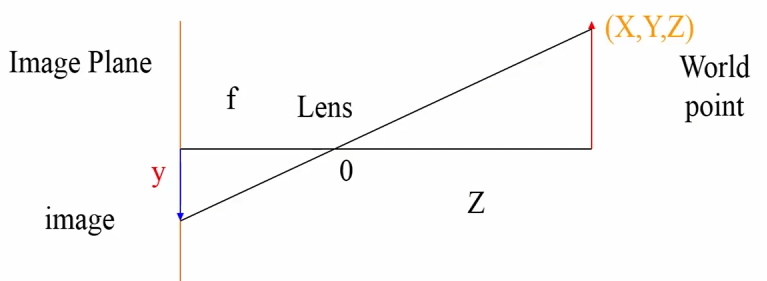
\includegraphics[scale=0.65]{perspective_lens.png}

\[\frac{-y}{Y}=\frac{f}{Z}\rightarrow y=-\frac{fY}{Z}\quad\quad \frac{-x}{X}=\frac{f}{Z}\rightarrow x =-\frac{fX}{Z}\]

\subsubsection*{Origin at the image center}
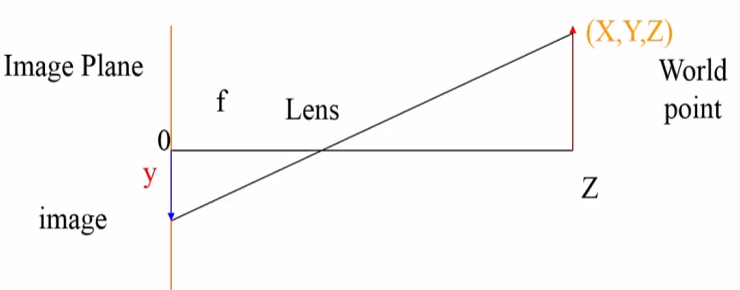
\includegraphics[scale=0.5]{perspective_image.png}

\[\frac{-y}{Y}=\frac{f}{Z-f}\rightarrow y=-\frac{fY}{Z-f}\quad\quad \frac{-x}{X}=\frac{f}{Z-f}\rightarrow x =-\frac{fX}{Z-f}\]

\section*{Transformations}
\subsection*{3D Translation}
\[\begin{bmatrix}
    X_2 \\ Y_2 \\ Z_2
\end{bmatrix} = \begin{bmatrix}
    X_1 \\ Y_1 \\ Z_1
\end{bmatrix} + \begin{bmatrix}
    d_x \\ d_y \\ d_z
\end{bmatrix}\]

\[\begin{bmatrix}
    X_2 \\ Y_2 \\ Z_2 \\ 1
\end{bmatrix} = T \begin{bmatrix}
    X_1 \\ Y_1 \\ Z_1 \\ 1
\end{bmatrix}\] where $T=\begin{bmatrix}
    1 & 0 & 0 & d_x \\
    0 & 1 & 0 & d_y \\
    0 & 0 & 1 & d_z \\
    0 & 0 & 0 & 1
\end{bmatrix}$ is the translation matrix

\subsection*{Scaling}
\[\begin{bmatrix}
    X_2 \\ Y_2 \\ Z_2
\end{bmatrix} = \begin{bmatrix}
    X_1 \times S_x \\ Y_1 \times S_y \\ Z_1 \times S_z
\end{bmatrix}\]

\[\begin{bmatrix}
    X_2 \\ Y_2 \\ Z_2 \\ 1
\end{bmatrix} = S \begin{bmatrix}
    X_1 \\ Y_1 \\ Z_1 \\ 1
\end{bmatrix}\] where $S=\begin{bmatrix}
    S_x & 0 & 0 & 0 \\
    0 & S_y & 0 & 0 \\
    0 & 0 & S_z & 0 \\
    0 & 0 & 0 & 1
\end{bmatrix}$ is the scaling matrix

\subsection*{Rotation}
Rotation matrices are orthonormal matrices, so the inverse and transpose of a rotation matrix are equal.
\[r_i \cdot r_j = \begin{cases}
    1 & \text{if } i = j \\
    0 & \text{otherwise}
\end{cases}\] where $r_i$ and $r_j$ are rows in the rotation matrix.

\vspace{1em}

\subsubsection*{Rotation around $Z$ axis:}
\[\begin{bmatrix}
    X_2 \\ Y_2 \\ Z_2
\end{bmatrix} = R \begin{bmatrix}
    X_1 \\ Y_1 \\ Z_1
\end{bmatrix}\] where $R=\begin{bmatrix}
    \cos\theta & -\sin\theta & 0 \\
    \sin\theta & \cos\theta & 0 \\
    0 & 0 & 1
\end{bmatrix}$ is the rotation matrix

\subsubsection*{Rotation around an arbitrary axis:}
\[R=R_Z^\alpha R_Y^\beta R_Z^\gamma=\begin{bmatrix}
    \cos\alpha\cos\beta & \cos\alpha\sin\beta\sin\gamma - \sin\alpha\cos\gamma & \cos\alpha\sin\beta\cos\gamma + \sin\alpha\sin\gamma \\
    \sin\alpha\cos\beta & \sin\alpha\sin\beta\sin\gamma + \cos\alpha\cos\gamma & \sin\alpha\sin\beta\cos\gamma - \cos\alpha\sin\gamma \\
    -\sin\beta & \cos\beta\sin\gamma & \cos\beta\cos\gamma
\end{bmatrix}\]

The approximation if angles are small ($\cos\theta \approx 1$) is:
\[\begin{bmatrix}
    1 & -\alpha & \beta \\
    \alpha & 1 & -\gamma \\
    -\beta & \gamma & 1
\end{bmatrix}\]

\subsection*{Perspective}
\textbf{Homogenous transformation}
\[(X, Y, Z) \rightarrow (kX, kY, kZ, k)\]
\textbf{Inverse Homogenous transformation}
\[(C_{h1}, C_{h2}, C_{h3}, C_{h4}) \rightarrow \Big(\frac{C_{h1}}{C_{h4}}, \frac{C_{h2}}{C_{h4}}, \frac{C_{h3}}{C_{h4}}\Big)\]

\[\begin{bmatrix}
    C_{h1} \\ C_{h2} \\ C_{h3} \\ C_{h4}
\end{bmatrix} = P \begin{bmatrix}
    kX \\ kY \\ kZ \\ k
\end{bmatrix}=\begin{bmatrix}
    kX \\ kY \\ kZ \\ k - \frac{kZ}{f}
\end{bmatrix}\] where $P=\begin{bmatrix}
    1 & 0 & 0 & 0 \\
    0 & 1 & 0 & 0 \\
    0 & 0 & 1 & 0 \\
    0 & 0 & \frac{-1}{f} & 1
\end{bmatrix}$ is the perspective matrix

\[x=\frac{C_{h1}}{C_{h4}}=\frac{kX}{k-\frac{kZ}{f}}=\frac{fX}{f-Z}\]
\[y=\frac{C_{h2}}{C_{h4}}=\frac{kY}{k-\frac{kZ}{f}}=\frac{fY}{f-Z}\]

\section*{Camera Model}
\begin{enumerate}
    \item Camera is at the origin of the world coordinates
    \item Translate by $G$
    \item Rotate around $Z$ axis in counter clockwise direction
    \item Rotate again around $X$ in counter clockwise direction
    \item Translate by $C$
\end{enumerate}
Since we are moving the camera instead of object we need to use inverse transformations.
\[C_h=P T_C R_{-\phi}^X R_{-\theta}^Z T_G W_h\]

Using the previous values for $P$, $C$, and $R$:
\[x=f\frac{(X-X_0)\cos\theta + (Y-Y_0)\sin\theta - r_1}{-(X-X_0)\sin\theta\sin\phi + (Y-Y_0)\cos\theta\sin\phi - (Z-Z_0)\cos\phi + r_3 + f}\]
\[y=f\frac{(X-X_0)\sin\theta\cos\phi + (Y-Y_0)\cos\theta\cos\phi + (Z-Z_0)\sin\phi - r_2}{-(X-X_0)\sin\theta\sin\phi + (Y-Y_0)\cos\theta\sin\phi - (Z-Z_0)\cos\phi + r_3 + f}\]

\subsection*{Camera Calibration}

Finding the $A$ matrix using 3D points and corresponding 2D points.
\[C_h=AW_h\]
\[\begin{bmatrix}
    Ch_1 \\ Ch_2 \\ Ch_3 \\ Ch_4
\end{bmatrix} = \begin{bmatrix}
    a_{11} & a_{12} & a_{13} & a_{14} \\
    a_{21} & a_{22} & a_{23} & a_{24} \\
    a_{31} & a_{32} & a_{33} & a_{34} \\
    a_{41} & a_{42} & a_{43} & a_{44}
\end{bmatrix}\begin{bmatrix}
    X \\ Y \\ Z \\ 1
\end{bmatrix}\]

\[Ch_1 = a_{11}X + a_{12}Y + a_{13}Z + a_{14} = Ch_4 x\]
\[Ch_2 = a_{21}X + a_{22}Y + a_{23}Z + a_{24} = Ch_4 y\]
\[Ch_4 = a_{41}X + a_{42}Y + a_{43}Z + a_{44}\]

\[x = \frac{C_{h1}}{C_{h4}} \quad y = \frac{C_{h2}}{C_{h4}}\]

\textbf{Solve for matrix using least squares fit.}

\begin{enumerate}
    \item Using the value for $Ch_4$ in terms of the unknown variables.
    \[a_{11}X + a_{12}Y + a_{13}Z + a_{14} - a_{41}Xx - a_{42}Yx - a_{43}Zx - a_{44}x = 0\]
    \[a_{21}X + a_{22}Y + a_{23}Z + a_{24} - a_{41}Xy - a_{42}Yy - a_{43}Zy - a_{44}y = 0\]
    \item Since the two equations are for one point, you can solve for the unknown values with enough points.
\end{enumerate}

\end{document}